\documentclass[tikz,border=6pt]{standalone}
\usepackage[T1]{fontenc}
\usepackage{amsmath}
\usetikzlibrary{arrows.meta,positioning,calc}
\begin{document}
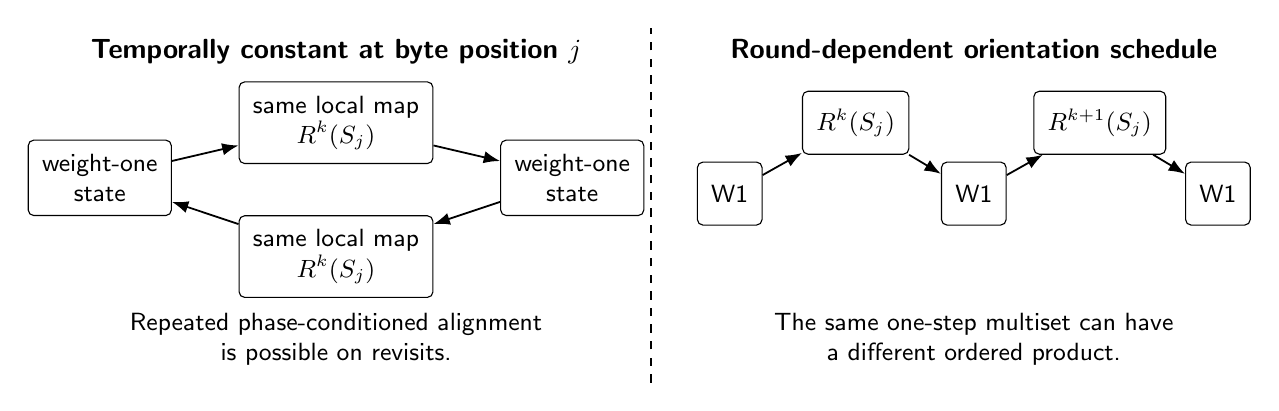
\begin{tikzpicture}[font=\sffamily\small,>=Latex,
 state/.style={draw,rounded corners=2pt,align=center,inner sep=5pt,minimum height=8mm},
 arr/.style={->,line width=.65pt}]
\node[font=\sffamily\bfseries] at (0,3.2) {Temporally constant at byte position $j$};
\node[state] (a1) at (-3,1.6) {weight-one\\state};
\node[state] (a2) at (0,2.3) {same local map\\$R^k(S_j)$};
\node[state] (a3) at (3,1.6) {weight-one\\state};
\node[state] (a4) at (0,.6) {same local map\\$R^k(S_j)$};
\draw[arr] (a1)--(a2); \draw[arr] (a2)--(a3); \draw[arr] (a3)--(a4); \draw[arr] (a4)--(a1);
\node[align=center] at (0,-.45) {Repeated phase-conditioned alignment\\is possible on revisits.};

\draw[dashed] (4,-1) -- (4,3.5);
\node[font=\sffamily\bfseries] at (8.1,3.2) {Round-dependent orientation schedule};
\node[state] (b1) at (5.0,1.4) {W1};
\node[state] (b2) at (6.6,2.3) {$R^k(S_j)$};
\node[state] (b3) at (8.1,1.4) {W1};
\node[state] (b4) at (9.7,2.3) {$R^{k+1}(S_j)$};
\node[state] (b5) at (11.2,1.4) {W1};
\draw[arr] (b1)--(b2); \draw[arr] (b2)--(b3); \draw[arr] (b3)--(b4); \draw[arr] (b4)--(b5);
\node[align=center] at (8.1,-.45) {The same one-step multiset can have\\a different ordered product.};
\end{tikzpicture}
\end{document}
